% Provenance (never printed): see sources/outline_sources.md (Year 3:
% facies analysis, depositional models, Walther's law, well logs). Brief:
% sources/book5/BRIEFS.md, ch. 17. Curves from figdata/bachelor-3/well_logs.py
% (unit tops from figdata/shared/region.py). Exercise and problem values in
% the Book 5 scratch calculator calc/ch17.py. The well Varden-2, its logs and
% the channel architecture of its sandstone are invented.
\chapter{Modelos de fácies}\label{ch:b3:facies-models}

Um testemunho de um poço com um quilômetro de profundidade: um metro de areia grossa com
estratificação cruzada, apoiada sobre uma base abrupta, que se torna para cima um silte com
vestígios de raízes, e depois areia de novo sobre outra base abrupta. O geólogo lê um rio que
serpenteou por sua planície, embora nenhum rio corra ali hoje. A leitura apoia-se em duas
ferramentas: um conjunto de modelos, cada um um resumo de muitos exemplos modernos e antigos
de um mesmo ambiente, e uma lei que transforma uma sucessão vertical de camadas em um mapa
de ambientes vizinhos.

\begin{recall}
Fácies sedimentares, ambiente de deposição, formas de leito, estratificação cruzada,
deltas dos três tipos, correntes de turbidez, turbiditos e camadas com gradação estão no
volume do primeiro ano, no capítulo sobre sedimentos clásticos e seus ambientes; a fábrica
carbonática, os recifes e as plataformas carbonáticas, no capítulo sobre sedimentos
carbonáticos, silicosos e evaporíticos; o perfil de sondagem e a correlação de perfis, no
capítulo sobre seções geológicas. Porosidade e
permeabilidade estão nos livros escolares. \omterm{def:b3:sequence-stratigraphy:parasequence}{Parassequências}, \omterm{def:b3:sequence-stratigraphy:parasequence}{superfícies de inundação} e
\omterm{def:b3:sequence-stratigraphy:tract}{tratos de sistemas} estão no capítulo~\ref{ch:b3:sequence-stratigraphy}. As ondas em águas profundas, cujo
movimento se atenua com a profundidade, estão nos volumes de física.
\end{recall}

\section{Fácies, sucessões e a lei de Walther}\label{sec:b3:facies-models:walther}

Uma fácies sedimentar descreve-se a partir do que se vê em um testemunho ou em um
penhasco: granulometria, seleção, estruturas, fósseis, cor. Uma única fácies raramente é
diagnóstica: areia com estratificação cruzada forma-se em rios, em praias, em canais de maré e
em desertos. O que identifica um ambiente é a companhia que a fácies mantém e a ordem em que
as fácies se sucedem.

\begin{definition}[Associação de fácies e sucessão de fácies]\label{def:b3:facies-models:association}
Uma \emph{associação de fácies}\index{associação de fácies} é um grupo de fácies
que ocorrem juntas e foram depositadas em um mesmo ambiente, como areia de canal, silte de dique
marginal e lama de planície de inundação com raízes. Uma \emph{sucessão de
fácies}\index{sucessão de fácies} é uma sequência vertical de fácies na qual alguma propriedade
muda progressivamente para cima; em uma \emph{sucessão com granodecrescência
ascendente}\index{sucessão com granodecrescência ascendente} a granulometria diminui para cima,
e em uma \emph{sucessão com granocrescência ascendente}\index{sucessão com granocrescência ascendente}
ela aumenta.
\end{definition}

\begin{definition}[Modelo de fácies]\label{def:b3:facies-models:model}
Um \emph{modelo de fácies}\index{modelo de fácies} é um resumo geral de um
ambiente de deposição, extraído de muitos exemplos modernos e antigos: as fácies que produz,
sua geometria, suas relações laterais e as sucessões que constroem. Ele serve como norma
para comparar um novo exemplo, como guia para observações adicionais, como preditor em
situações novas e como base para
interpretar o ambiente.
\end{definition}

A ponte entre o lateral e o vertical é uma lei. Ambientes vizinhos situam-se lado a lado
a qualquer momento: a praia ao lado da \omterm{def:b3:facies-models:shoreface}{antepraia}, a \omterm{def:b3:facies-models:shoreface}{antepraia} ao lado da lama de mar
aberto. Quando a linha de costa se desloca,
cada ambiente passa a jazer sobre o seu vizinho.

\begin{theorem}[Lei de Walther]\label{thm:b3:facies-models:walther}
Em uma sucessão concordante, sem uma quebra significativa na deposição nem uma superfície erosiva,
as fácies que se situam diretamente umas sobre as outras foram depositadas
em ambientes que estavam lado a lado na época.
\end{theorem}

\begin{proof}
Consideram-se cinturões de ambientes, cada um uma faixa paralela à linha de costa, que
migram juntos através da bacia enquanto o assoalho subside ou o nível do mar sobe.
Em um lugar fixo, os cinturões passam um após o outro, na ordem em que estão lado a lado,
e cada um deixa seu depósito sobre o depósito do cinturão que o precedeu. Se a deposição
é contínua, a ordem vertical dos depósitos é, portanto, a ordem lateral dos cinturões.
Uma quebra ou uma superfície de erosão interrompe o argumento:
os cinturões que passaram durante a lacuna não deixaram nada, ou
seus depósitos foram removidos, e fácies de ambientes não adjacentes
entram em contato.
\end{proof}

\begin{omfigure}
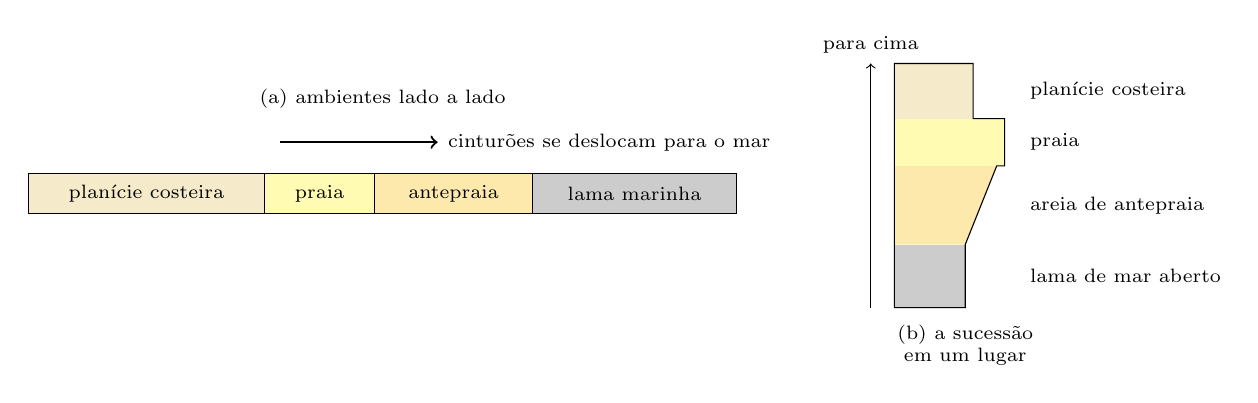
\begin{tikzpicture}[font=\scriptsize, x=1cm, y=1cm]
% environments side by side, with a shoreline that moves seaward
\fill[yellow!35!brown!25] (0,0) rectangle (3,0.5);
\fill[yellow!30] (3,0) rectangle (4.4,0.5);
\fill[yellow!50!orange!30] (4.4,0) rectangle (6.4,0.5);
\fill[black!20] (6.4,0) rectangle (9,0.5);
\draw (0,0) rectangle (9,0.5);
\foreach \x in {3,4.4,6.4} {\draw (\x,0) -- (\x,0.5);}
\node at (1.5,0.25) {planície costeira};
\node at (3.7,0.25) {praia};
\node at (5.4,0.25) {antepraia};
\node at (7.7,0.25) {lama marinha};
\draw[->, thick] (3.2,0.9) -- (5.2,0.9) node[right] {cinturões se deslocam para o mar};
\node[anchor=south] at (4.5,1.2) {(a) ambientes lado a lado};
% vertical succession at a place
\begin{scope}[xshift=11cm, yshift=-1.2cm]
\fill[black!20] (0,0) rectangle (0.9,0.8);
\fill[yellow!50!orange!30] (0,0.8) -- (0.9,0.8) -- (1.3,1.8) -- (0,1.8) -- cycle;
\fill[yellow!30] (0,1.8) rectangle (1.4,2.4);
\fill[yellow!35!brown!25] (0,2.4) rectangle (1.0,3.1);
\draw (0,0) -- (0.9,0) -- (0.9,0.8) -- (1.3,1.8) -- (1.4,1.8) -- (1.4,2.4) -- (1.0,2.4) -- (1.0,3.1) -- (0,3.1) -- cycle;
\node[anchor=west] at (1.6,0.4) {lama de mar aberto};
\node[anchor=west] at (1.6,1.3) {areia de antepraia};
\node[anchor=west] at (1.6,2.1) {praia};
\node[anchor=west] at (1.6,2.75) {planície costeira};
\draw[->] (-0.3,0) -- (-0.3,3.1) node[above] {para cima};
\node[anchor=north, align=center] at (0.9,-0.1) {(b) a sucessão\\ em um lugar};
\end{scope}
\end{tikzpicture}

\par\smallskip{\small A lei de Walther. (a) Os ambientes situam-se lado a lado ao longo
de um perfil; (b) à medida que os cinturões avançam para o mar, um lugar recebe lama de mar aberto,
depois areia de \omterm{def:b3:facies-models:shoreface}{antepraia}, areia de praia e depósitos de planície costeira: uma
\omterm{def:b3:facies-models:association}{sucessão com granocrescência ascendente}, na ordem dos cinturões (a largura no perfil
indica granulometria mais grossa).}\label{fig:b3:facies-models:walther}
\end{omfigure}

A lei funciona nos dois sentidos. Uma regressão empilha os cinturões na sua ordem em direção ao mar
para cima, e uma transgressão, na ordem inversa; e uma sucessão vertical lida em um testemunho
fornece o mapa dos ambientes vizinhos à época. Ela falha exatamente
onde o Capítulo~\ref{ch:b3:sequence-stratigraphy} situa suas superfícies-chave:
através de um \omterm{def:b3:sequence-stratigraphy:sequence}{limite de sequência}, onde a exposição e a erosão levam areia fluvial
sobre lama de plataforma, e através de uma \omterm{def:b3:sequence-stratigraphy:parasequence}{superfície de inundação}, onde a lama de mar aberto repousa diretamente sobre
a planície costeira.

\section{Rios}\label{sec:b3:facies-models:rivers}

\begin{definition}[Rios entrelaçados e meandrantes]\label{def:b3:facies-models:rivers}
Um \emph{rio entrelaçado}\index{rio entrelaçado} escoa em vários canais rasos
que se dividem e se reúnem em torno de barras, sobre uma planície íngreme, onde há
abundante carga grossa e vazão variável. Um \emph{rio meandrante}\index{rio meandrante}
escoa em um único canal sinuoso sobre uma planície mais suave, transportando mais
sedimento fino; ele migra erodindo a margem externa de cada curva e depositando na
margem interna. O depósito da margem interna é uma \emph{barra de
pontal}\index{barra de pontal}. A \emph{avulsão}\index{avulsão} é o abandono de
um canal para um novo curso através da planície de inundação, geralmente depois que uma
cheia rompe um dique marginal.
\end{definition}

Uma \omterm{def:b3:facies-models:rivers}{barra de pontal} cresce lateralmente à medida que a curva migra, de modo que em qualquer lugar ela registra
a seção transversal do canal da base ao topo: uma lag formada pelos clastos mais grossos
sobre uma base erosiva, areia com estratificação cruzada vinda das dunas do
canal profundo, areia mais fina com marcas onduladas do topo raso da barra e, em seguida,
o silte e a lama da planície de inundação, com raízes e solos. Pela lei de Walther
esta \omterm{def:b3:facies-models:association}{sucessão com granodecrescência ascendente}, com alguns metros de espessura, tem a
espessura da profundidade do canal. Um \omterm{def:b3:facies-models:rivers}{rio entrelaçado} deixa lençóis empilhados de areia com estratificação cruzada
e cascalho com pouca lama, cuja granulometria quase não muda para cima; seus finos são
levados embora. A \omterm{def:b3:facies-models:rivers}{avulsão} desloca o cinturão de canais pela planície, de modo que
os corpos de canal se empilham ao acaso entre lamas de planície de inundação, separados por
bases erosivas nítidas.

\begin{omfigure}
\begin{tikzpicture}[font=\scriptsize, x=1cm, y=1cm]
% (a) braided plan
\begin{scope}
\fill[yellow!35!brown!20] (0,0) rectangle (4.6,2.4);
\draw[omDef!60, line width=1.6pt] (0,1.2) .. controls (0.8,1.6) and (1.4,0.6) .. (2.3,1.0) .. controls (3.0,1.3) and (3.6,0.7) .. (4.6,1.0);
\draw[omDef!60, line width=1.6pt] (0,1.2) .. controls (0.8,0.8) and (1.6,1.9) .. (2.4,1.6) .. controls (3.2,1.3) and (3.8,1.9) .. (4.6,1.6);
\draw[omDef!60, line width=1.2pt] (1.2,1.25) .. controls (1.8,1.5) and (2.6,1.2) .. (3.3,1.35);
\fill[yellow!45] (1.5,1.15) ellipse (0.35 and 0.12);
\fill[yellow!45] (3.0,1.25) ellipse (0.4 and 0.12);
\node[anchor=south] at (2.3,2.45) {(a) entrelaçado};
\end{scope}
% (b) meandering plan
\begin{scope}[xshift=5.4cm]
\fill[green!30!black!12] (0,0) rectangle (4.6,2.4);
\draw[omDef!60, line width=2pt] (0,1.2) .. controls (0.6,2.2) and (1.4,2.2) .. (1.6,1.2) .. controls (1.8,0.2) and (2.8,0.2) .. (3.0,1.2) .. controls (3.2,2.2) and (4.0,2.2) .. (4.6,1.2);
\fill[yellow!45] (0.8,1.45) ellipse (0.3 and 0.2);
\fill[yellow!45] (2.3,0.95) ellipse (0.3 and 0.2);
\fill[yellow!45] (3.8,1.45) ellipse (0.3 and 0.2);
\node at (2.3,0.95) {pb};
\draw[omDef!40, line width=1pt, densely dashed] (0.4,0.2) .. controls (1.0,0.7) and (1.6,0.4) .. (2.0,0.1);
\node[anchor=west, font=\tiny] at (2.6,2.15) {planície de inundação};
\node[anchor=south] at (2.3,2.45) {(b) meandrante};
\end{scope}
% logs
\begin{scope}[xshift=10.8cm]
\fill[yellow!45] (0,0) -- (1.2,0) -- (1.2,2.0) -- (0,2.0) -- cycle;
\draw (0,0) -- (1.2,0) -- (1.15,0.6) -- (1.2,0.65) -- (1.1,1.3) -- (1.2,1.35) -- (1.15,2.0) -- (0,2.0) -- cycle;
\node[anchor=north] at (0.6,-0.05) {entrelaçado};
\end{scope}
\begin{scope}[xshift=12.6cm]
\fill[yellow!45] (0,0) -- (1.2,0) -- (1.1,0.9) -- (0.45,1.6) -- (0,1.6) -- cycle;
\fill[green!30!black!15] (0,1.6) rectangle (0.3,2.2);
\draw (0,0) -- (1.2,0) -- (1.1,0.9) -- (0.45,1.6) -- (0.3,1.6) -- (0.3,2.2) -- (0,2.2) -- cycle;
\draw[decorate, decoration={snake, amplitude=0.4mm, segment length=1.5mm}] (0,0) -- (1.2,0);
\node[anchor=north] at (0.6,-0.05) {barra de pontal};
\node[anchor=west, font=\tiny] at (0.35,1.9) {raízes};
\end{scope}
\end{tikzpicture}

\par\smallskip{\small (a) Um \omterm{def:b3:facies-models:rivers}{rio entrelaçado}: vários canais em torno de barras de
areia e cascalho. (b) Um \omterm{def:b3:facies-models:rivers}{rio meandrante}: um único canal sinuoso, \omterm{def:b3:facies-models:rivers}{barras de pontal} (pb)
nas margens internas, um curso abandonado (tracejado) deixado pela \omterm{def:b3:facies-models:rivers}{avulsão}. À direita:
perfis granulométricos dos depósitos (a largura indica granulometria mais grossa): lençóis de areia empilhados
com pouca variação para cima, no caso do \omterm{def:b3:facies-models:rivers}{rio entrelaçado}, e uma \omterm{def:b3:facies-models:association}{sucessão com granodecrescência ascendente}, de base nítida
capeada por lama de planície de inundação com raízes, no caso da
\omterm{def:b3:facies-models:rivers}{barra de pontal}.}\label{fig:b3:facies-models:rivers}
\end{omfigure}

\section{Litorais, deltas e plataformas}\label{sec:b3:facies-models:shelves}

Os deltas do volume do primeiro ano, dominados por rios, ondas ou marés, constroem-se todos
pelo mesmo mecanismo: a desembocadura deposita sua carga onde a corrente diminui, e a frente deltaica
prograda sobre suas próprias lamas de pró-delta. Uma
frente deltaica ou \omterm{def:b3:facies-models:shoreface}{antepraia} em progradação deixa, pela lei de Walther, uma
\omterm{def:b3:facies-models:association}{sucessão com granocrescência ascendente}: lama de mar aberto, lama intercalada com areia de
tempestade, areia de \omterm{def:b3:facies-models:shoreface}{antepraia}, praia. Cada \omterm{def:b3:sequence-stratigraphy:parasequence}{parassequência} do capítulo anterior é uma
dessas sucessões.

\begin{definition}[Antepraia e bases de ondas]\label{def:b3:facies-models:shoreface}
A \emph{antepraia}\index{antepraia} é a zona inclinada situada do lado do mar, em relação à
praia, onde as ondas retrabalham continuamente o fundo do mar. Sua base é a
\emph{base das ondas de tempo bom}\index{base das ondas de tempo bom}, a profundidade abaixo da
qual as ondas comuns não movem mais o sedimento do fundo. A \emph{base das ondas de
tempestade}\index{base das ondas de tempestade} é o limite mais profundo atingido pelas ondas de tempestade;
entre as duas, a lama assenta em tempo calmo e é retrabalhada em camadas de areia
durante as tempestades. Abaixo da base das ondas de tempestade, o fundo não é perturbado pelas ondas.
\end{definition}

\begin{omfigure}
\begin{tikzpicture}[font=\scriptsize, x=1cm, y=1.6cm]
\fill[omSea!60] (0,2.2) -- (13,2.2) -- (13,0.2) -- (5.5,0.9) -- (2.0,1.9) -- (0.6,2.2) -- cycle;
\fill[yellow!40] (0,2.4) -- (0.6,2.2) -- (2.0,1.9) -- (5.5,0.9) -- (5.5,0.0) -- (0,0.0) -- cycle;
\fill[black!18] (5.5,0.9) -- (13,0.2) -- (13,0) -- (5.5,0) -- cycle;
\draw[thick] (0,2.4) -- (0.6,2.2) -- (2.0,1.9) -- (5.5,0.9) -- (13,0.2);
\draw[omDef] (0,2.2) -- (13,2.2);
\draw[omDef, densely dashed] (1.6,1.97) -- (13,1.97);
\draw[omDef, densely dashed] (5.5,0.9) -- (13,0.9);
\node[omDef, anchor=north west] at (9.3,1.95) {base das ondas de tempo bom};
\node[omDef, anchor=north west] at (9.3,0.88) {base das ondas de tempestade};
\node[anchor=south] at (0.5,2.42) {praia};
\node at (1.8,1.35) {antepraia};
\node at (4.3,0.45) {transição para o largo};
\node at (9.0,0.15) {lama de plataforma externa};
\node[align=center] at (7.4,1.45) {camadas de areia de tempestade,\\ estratificação cruzada hummocky};
\end{tikzpicture}

\par\smallskip{\small Perfil de costa dominada por ondas (esquemático, com escala vertical
muito exagerada). Acima da \omterm{def:b3:facies-models:shoreface}{base das ondas de tempo bom}, a areia da \omterm{def:b3:facies-models:shoreface}{antepraia} é retrabalhada
todos os dias; entre as duas bases de ondas, a lama alterna-se com camadas de areia depositadas
por tempestades; abaixo da \omterm{def:b3:facies-models:shoreface}{base das ondas de tempestade}, a lama
se acumula.}\label{fig:b3:facies-models:shoreface}
\end{omfigure}

O movimento orbital de uma onda em águas profundas decai como $e^{-2\pi z/\lambda}$
com a profundidade $z$, para um comprimento de onda $\lambda$: a meio comprimento de onda ela mantém
\qty{4}{\percent} de sua amplitude na superfície, o que define a escala de uma
base de ondas. Boias registraram mais de dois milhões de espectros de ondas no Caribe, no golfo do México e no oeste do Atlântico,
que fornecem comprimentos de onda modais de cerca de
\qty{75}{m} nos mares abrigados e de cerca de \qty{110}{m} na margem aberta,
e mostram que, quando calculados como médias ao longo de semanas a anos, os comprimentos de onda não se separam
em uma classe de tempo bom e uma classe de tempestade: a chance de uma onda agitar o fundo
cresce de forma contínua à medida que a lâmina d'água diminui. As duas bases de ondas continuam
sendo termos úteis para zonas de um perfil, não profundidades precisas.
% ledger: losspeters10:wavebase

\begin{definition}[Estratificação cruzada hummocky]\label{def:b3:facies-models:hcs}
A \emph{estratificação cruzada hummocky}\index{Estratificação cruzada hummocky} é uma estratificação de areia fina
em lâminas suavemente curvas, côncavas para cima (depressões) e convexas para cima (cumes), que se cortam
em baixos ângulos e engrossam e afinam lateralmente, em comprimentos de onda de um metro a vários metros. Ela
se forma pelos fluxos oscilatórios e combinados das ondas de tempestade, entre
a \omterm{def:b3:facies-models:shoreface}{base das ondas de tempo bom}
e a \omterm{def:b3:facies-models:shoreface}{base das ondas de tempestade}.
\end{definition}

\begin{inthefield}[Camadas de tempestade em uma plataforma siluriana]
\begin{minipage}[t]{0.42\linewidth}\vspace{0pt}
Na Formação Arisaig, em Nova Scotia, camadas de arenito fino separam
folhelhos mais escuros. Geólogos que estudaram essas camadas reconhecem as lâminas baixas, curvas
entrecruzadas da \omterm{def:b3:facies-models:hcs}{estratificação cruzada hummocky}: cada camada registra uma
tempestade que agitou a plataforma abaixo do alcance das ondas comuns, e a lama
ao seu redor registra a longa calmaria entre as tempestades.
\end{minipage}\hfill
\begin{minipage}[t]{0.54\linewidth}\vspace{0pt}
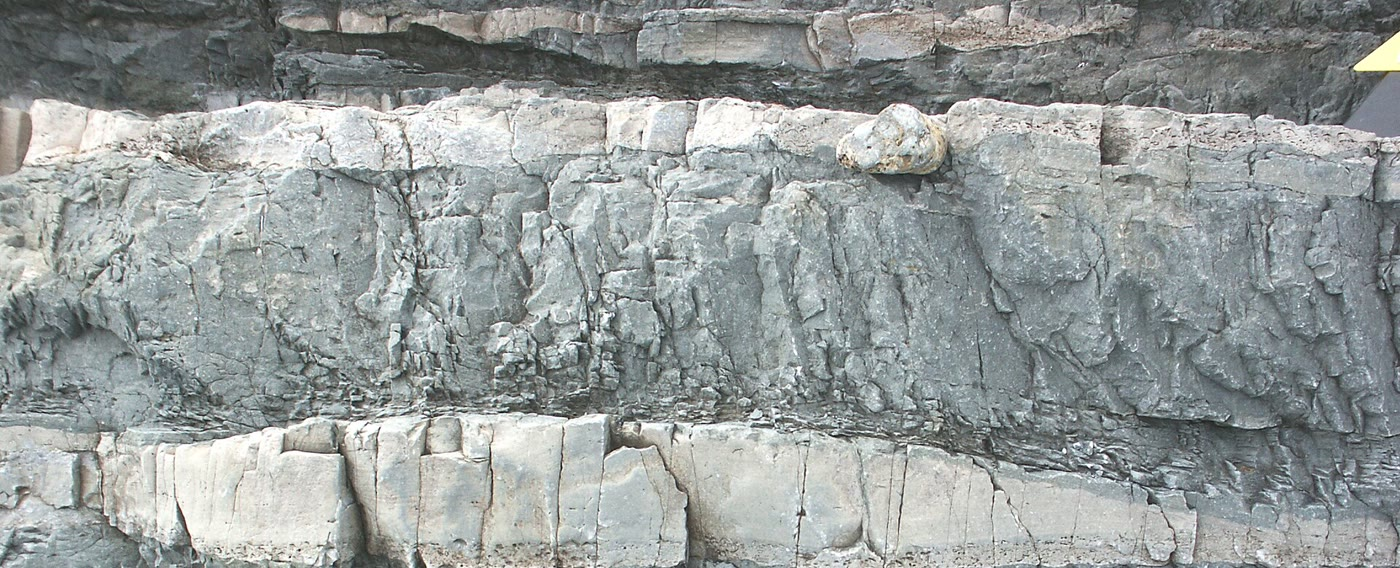
\includegraphics[width=\linewidth]{images/book5/b3-hummocky-cross-stratification.jpg}

{\scriptsize \omterm{def:b3:facies-models:hcs}{Estratificação cruzada hummocky} na Formação Arisaig
(siluriana), perto de Arisaig, Nova Scotia. Foto Michael C. Rygel, CC BY-SA 3.0
(recortada).}
\end{minipage}
\end{inthefield}
% ledger: photo:b3-hcs

Onde as marés dominam, as fácies mudam: correntes de enchente e de vazante constroem
estratificações cruzadas com sentidos opostos, cortinas de lama assentam-se a cada
águas paradas, e a espessura dos conjuntos entre as cortinas aumenta e diminui com
o ciclo de marés de sizígia e de quadratura. Canais de maré, planícies e cordões arenosos
têm modelos próprios, construídos da mesma forma.

\section{Águas profundas}\label{sec:b3:facies-models:deep}

Uma corrente de turbidez que desacelera deposita sua carga na ordem de sedimentação:
primeiro os grãos mais grossos, por último os mais finos. Uma camada completa de turbidito mostra
essa ordem em cinco divisões.

\begin{definition}[Sequência de Bouma]\label{def:b3:facies-models:bouma}
A \emph{sequência de Bouma}\index{sequência de Bouma} é a sucessão ideal de
divisões em uma camada de turbidito, da base ao topo: Ta, areia maciça ou gradada sobre
uma base erosiva com marcas de sulco e de ferramenta; Tb, areia com laminação paralela; Tc,
areia fina com laminação cruzada de marcas onduladas e convoluta; Td, silte com laminação paralela;
Te, lama, em parte da corrente de turbidez e em parte da lenta sedimentação
entre os fluxos.
\end{definition}

Poucas camadas mostram as cinco: perto da fonte a corrente é rápida e deixa divisões Ta espessas
com as superiores erodidas pelo fluxo seguinte; longe dela chegam apenas
as divisões mais finas, de Tc a Te. A sequência registra, assim, o
declínio de um fluxo, e a mudança das camadas ao longo do leque registra o declínio dos
fluxos com a distância.

\begin{definition}[Leque submarino]\label{def:b3:facies-models:fan}
Um \emph{leque submarino}\index{leque submarino} é um cone de sedimento na base
de um talude continental, alimentado por um cânion: um leque superior com um canal principal
entre diques marginais, um leque médio de canais distributários que terminam em lobos arenosos,
e um leque inferior de turbiditos delgados que passam a lama do assoalho da bacia.
\end{definition}

Ao longo da margem, correntes profundas impulsionadas pela circulação oceânica retrabalham o
sedimento fino do talude em contorritos, montes e \textit{drifts}
silte e lama bioturbados que crescem ao longo das isóbatas, e não
encosta abaixo.

\begin{omfigure}
\begin{tikzpicture}[font=\scriptsize, x=1cm, y=1cm]
% (a) Bouma log
\begin{scope}
\fill[yellow!45] (0,0) -- (1.6,0) -- (1.6,1.2) -- (0,1.2) -- cycle;
\fill[yellow!35] (0,1.2) rectangle (1.3,1.8);
\fill[yellow!25] (0,1.8) rectangle (1.0,2.4);
\fill[black!12] (0,2.4) rectangle (0.7,2.8);
\fill[black!25] (0,2.8) rectangle (0.4,3.3);
\draw (0,0) -- (1.6,0) -- (1.6,1.2) -- (1.3,1.2) -- (1.3,1.8) -- (1.0,1.8) -- (1.0,2.4) -- (0.7,2.4) -- (0.7,2.8) -- (0.4,2.8) -- (0.4,3.3) -- (0,3.3) -- cycle;
\draw[decorate, decoration={snake, amplitude=0.5mm, segment length=2mm}] (0,0) -- (1.6,0);
\foreach \y in {1.35,1.5,1.65} {\draw[black!60] (0.05,\y) -- (1.25,\y);}
\foreach \x in {0.15,0.45,0.75} {\draw[black!60] (\x,1.95) .. controls (\x+0.08,2.1) .. (\x+0.2,1.95);}
\foreach \y in {2.5,2.6,2.7} {\draw[black!60] (0.05,\y) -- (0.65,\y);}
\foreach \y/\t in {0.6/Ta, 1.5/Tb, 2.1/Tc, 2.6/Td, 3.05/Te} {\node[anchor=west] at (1.9,\y) {\t};}
\node[anchor=west, align=left, font=\tiny] at (2.4,0.6) {areia gradada ou maciça,\\ base erosiva};
\node[anchor=west, font=\tiny] at (2.4,1.5) {laminação paralela};
\node[anchor=west, font=\tiny] at (2.4,2.1) {marcas onduladas, laminação convoluta};
\node[anchor=west, font=\tiny] at (2.4,2.6) {silte laminado};
\node[anchor=west, font=\tiny] at (2.4,3.05) {lama};
\node[anchor=north] at (1.6,-0.15) {(a) uma camada de turbidito};
\end{scope}
% (b) fan plan
\begin{scope}[xshift=8.2cm, yshift=0.2cm]
\fill[black!8] (-1.0,-0.2) rectangle (5.6,3.1);
\fill[yellow!20] (0.3,2.9) .. controls (1.6,2.6) and (4.9,2.0) .. (5.2,0.9) .. controls (4.6,-0.1) and (1.2,0.1) .. (0.3,1.6) -- cycle;
\fill[yellow!45] (1.9,1.9) ellipse (0.55 and 0.3);
\fill[yellow!45] (2.6,1.0) ellipse (0.55 and 0.3);
\fill[yellow!45] (3.4,1.75) ellipse (0.5 and 0.28);
\draw[omDef, line width=1.4pt] (-0.9,3.0) .. controls (-0.3,2.8) and (0.4,2.6) .. (1.0,2.2);
\draw[omDef, line width=0.8pt] (1.0,2.2) -- (1.6,1.95);
\draw[omDef, line width=0.8pt] (1.0,2.2) -- (2.3,1.15);
\draw[omDef, line width=0.8pt] (1.0,2.2) .. controls (2.0,2.4) .. (3.1,1.85);
\node[anchor=south west] at (-0.95,3.0) {cânion};
\node[anchor=east] at (0.55,2.0) {diques marginais};
\node[align=center, font=\tiny] at (2.6,1.0) {lobo};
\node at (4.4,0.7) {leque inferior};
\node[black!60] at (4.9,2.85) {assoalho da bacia};
\node[anchor=north] at (2.3,-0.25) {(b) um leque submarino em planta};
\end{scope}
\end{tikzpicture}

\par\smallskip{\small (a) A \omterm{def:b3:facies-models:bouma}{sequência de Bouma} de um leito completo de turbidito,
desenhada como perfil de granulometria (largura significa granulação mais grossa), com suas cinco divisões. (b)
Um \omterm{def:b3:facies-models:fan}{leque submarino} em planta: um cânion alimenta um canal entre diques marginais, que
se divide em canais distributários terminando em lobos de areia; turbiditos delgados
espalham-se sobre o leque inferior.}\label{fig:b3:facies-models:deep}
\end{omfigure}

\section{Plataformas carbonáticas}\label{sec:b3:facies-models:carbonates}

O sedimento carbonático é produzido no local onde se encontra, por organismos em água quente, límpida
e rasa, e suas fácies seguem o perfil da plataforma que a
fábrica carbonática constrói para si mesma.

\begin{definition}[Rampa carbonática e plataforma com borda]\label{def:b3:facies-models:ramp}
Uma \emph{rampa carbonática}\index{rampa carbonática} é uma plataforma cujo assoalho
inclina-se suave e uniformemente desde a linha de costa até a bacia, sem nenhuma quebra:
seus cinturões de fácies, desde planícies de maré e areias de barreiras de praia até grãos de
baixio, areia bioclástica e lama calcária de águas profundas, são largos e passam gradualmente uns
para os outros, selecionados pela energia das ondas, que diminui com a profundidade. Uma \emph{plataforma com
borda}\index{plataforma com borda} é uma plataforma de topo plano com uma quebra
de declive marcada em sua margem, onde recifes e bancos de areia constroem uma borda que abriga
uma laguna atrás dela; além da borda, um talude íngreme despeja blocos e grãos
na bacia.
\end{definition}

\begin{omfigure}
\begin{tikzpicture}[font=\scriptsize, x=1cm, y=1cm]
\begin{scope}
\fill[omSea!60] (0,1.6) -- (6.4,1.6) -- (6.4,0.3) -- cycle;
\fill[black!10] (0,1.6) -- (6.4,0.3) -- (6.4,0) -- (0,0) -- cycle;
\draw[thick] (0,1.7) -- (0.3,1.6) -- (6.4,0.3);
\draw[omDef] (0,1.6) -- (6.4,1.6);
\node[anchor=south] at (0.6,1.65) {planície de maré};
\node[rotate=-12, font=\tiny] at (1.5,1.08) {grãos de baixio};
\node[rotate=-12, font=\tiny] at (3.4,0.66) {areia bioclástica};
\node[rotate=-12, font=\tiny] at (5.3,0.26) {lama calcária};
\node[anchor=north, align=center] at (3.2,-0.1) {(a) rampa: declive uniforme,\\ cinturões graduais};
\end{scope}
\begin{scope}[xshift=7.2cm]
\fill[omSea!60] (0,1.6) -- (6.4,1.6) -- (6.4,0.2) -- (4.4,0.3) -- (3.6,1.55) -- (3.2,1.6) -- (0.3,1.6) -- cycle;
\fill[omSea!60] (0.3,1.6) -- (3.2,1.6) -- (3.0,1.35) -- (0.6,1.35) -- cycle;
\fill[black!10] (0,1.7) -- (0.3,1.6) -- (0.6,1.35) -- (3.0,1.35) -- (3.2,1.6) -- (3.6,1.55) -- (4.4,0.3) -- (6.4,0.2) -- (6.4,0) -- (0,0) -- cycle;
\draw[thick] (0,1.7) -- (0.3,1.6) -- (0.6,1.35) -- (3.0,1.35) -- (3.2,1.6) -- (3.6,1.55) -- (4.4,0.3) -- (6.4,0.2);
\fill[orange!50] (3.05,1.4) -- (3.2,1.6) -- (3.55,1.56) -- (3.6,1.4) -- cycle;
\draw[omDef] (0,1.6) -- (6.4,1.6);
\node at (1.8,1.12) {laguna};
\node[anchor=south] at (3.35,1.65) {borda de recife};
\node[anchor=west] at (4.2,0.95) {talude íngreme};
\node at (5.5,0.6) {bacia};
\node[anchor=north, align=center] at (3.2,-0.1) {(b) plataforma com borda: uma borda,\\ uma laguna, um talude};
\end{scope}
\end{tikzpicture}

\par\smallskip{\small Perfis de plataformas carbonáticas (esquemáticos, escala vertical
muito exagerada). (a) Uma rampa: cinturões selecionados pela energia das ondas ao longo de um
declive uniforme. (b) Uma \omterm{def:b3:facies-models:ramp}{plataforma com borda}: um recife e uma borda de bancos de grãos na quebra
de declive abrigam uma laguna de lama calcária; o talude além recebe blocos e grãos
desprendidos da borda.}\label{fig:b3:facies-models:platforms}
\end{omfigure}

Sobre o topo de uma plataforma plana, uma pequena elevação do nível relativo do mar inunda as
planícies de maré, e a fábrica, trabalhando mais rapidamente na água mais rasa, preenche
novamente o espaço até o nível do mar em pouco tempo. O resultado é uma pilha de
ciclos peritidais com um ou alguns metros de espessura, cada um uma \omterm{def:b3:sequence-stratigraphy:parasequence}{parassequência} de
raseamento ascendente, desde lama subtidal até uma planície de maré com fendas de dessecação ou
tapetes microbianos, coberta pela \omterm{def:b3:sequence-stratigraphy:parasequence}{superfície de inundação} seguinte.

\section{Testemunhos e perfis de poços}\label{sec:b3:facies-models:logs}

A maior parte da rocha sob as bacias sedimentares é conhecida por furos de sondagem. Poucos
são testemunhados, e seus testemunhos são descritos camada por camada, como um penhasco; quase todos
são perfilados.

\begin{definition}[Perfis a cabo]\label{def:b3:facies-models:wireline}
Um \emph{perfil a cabo}\index{perfil a cabo} é um registro contínuo de uma
propriedade física das rochas em função da profundidade, medido por uma sonda descida por
um cabo em um furo de sondagem. O \emph{perfil de raios gama}\index{perfil de raios gama}
registra a radiação gama natural da rocha, em unidades API: alta em
folhelho, cujas argilas contêm potássio, tório e urânio, baixa em areia quartzosa limpa
e em calcário. O \emph{perfil de densidade}\index{perfil de densidade}
registra a densidade aparente a partir do espalhamento de raios gama emitidos por uma
fonte na sonda. O \emph{perfil sônico}\index{perfil sônico} registra o
tempo de trânsito intervalar de uma onda compressional, em microssegundos por pé. O
\emph{perfil de nêutrons}\index{perfil de nêutrons} registra a desaceleração de nêutrons pelo
hidrogênio, e portanto a água retida nos poros e nas argilas.
\end{definition}
% ledger: keys:gamma, keys:density-porosity, keys:sonic

A unidade API de raios gama é definida em uma fossa de calibração: um duzentésimo da
diferença entre uma zona de radioatividade desprezível e uma zona com
os radioisótopos de um folhelho médio, a cerca do dobro de sua concentração. Carvão,
calcário e dolomito costumam ser menos radioativos que o folhelho; o arenito quartzoso é baixo, e um
arcóseo rico em feldspato potássico é mais alto; qualquer rocha pode tornar-se radioativa pelo
urânio carreado pela água subterrânea.
% ledger: keys:gamma

\begin{proposition}[Porosidade a partir da densidade e do tempo de trânsito]\label{prop:b3:facies-models:porosity}
Uma rocha de porosidade $\phi$, com grãos de densidade $\rho_{\mathrm{ma}}$ e
poros preenchidos por um fluido de densidade $\rho_f$, tem a densidade aparente
$\rho_b = (1 - \phi)\rho_{\mathrm{ma}} + \phi\rho_f$, de modo que
\[
\phi = \frac{\rho_{\mathrm{ma}} - \rho_b}{\rho_{\mathrm{ma}} - \rho_f}.
\]
Se uma onda compressional atravessa os grãos e o fluido em série, em
comprimentos proporcionais a $1 - \phi$ e $\phi$, seu tempo de trânsito é
$\Delta t = (1 - \phi)\Delta t_{\mathrm{ma}} + \phi\Delta t_f$ (a
equação da média temporal), e $\phi = (\Delta t - \Delta
t_{\mathrm{ma}})/(\Delta t_f - \Delta t_{\mathrm{ma}})$.
\end{proposition}

\begin{proof}
Um volume unitário de rocha contém um volume $1 - \phi$ de grãos e $\phi$ de
fluido; sua massa é $(1 - \phi)\rho_{\mathrm{ma}} + \phi\rho_f$, da qual se
isola $\phi$. Para a onda, um caminho de comprimento unitário atravessa $1 - \phi$ de
grãos e $\phi$ de fluido, e os tempos se somam.
\end{proof}

As densidades dos grãos são \qty{2.65}{g/cm^3} para o quartzo e \qty{2.71}{g/cm^3} para
o calcário; a água dos poros tem \qty{1.0}{g/cm^3} quando doce e até
\qty{1.1}{g/cm^3} como salmoura. Os tempos de trânsito variam de 42 a
\qty{48}{\micro\second/ft} na dolomita, de 48 a 53 no calcário, 53 para um
arenito consolidado, e 189 na salmoura. A equação da densidade é exata para
uma matriz conhecida; a equação da média temporal é uma regra empírica que funciona
melhor em rochas consolidadas com poros intergranulares. O folhelho quebra as duas:
as argilas têm densidades próprias e retêm água ligada.
% ledger: keys:density-porosity, keys:sonic

\begin{definition}[Razão net-to-gross]\label{def:b3:facies-models:ntg}
A \emph{razão net-to-gross}\index{razão net-to-gross} de um intervalo é a
espessura de sua rocha de qualidade de reservatório, geralmente areia identificada
no \omterm{def:b3:facies-models:wireline}{perfil de raios gama} abaixo de um valor de corte, dividida pela espessura total do intervalo.
\end{definition}

A forma da curva de raios gama através de um corpo arenoso é uma ferramenta de fácies.
Um \emph{sino}, limpo na base e mais argiloso para cima, indica uma
\omterm{def:b3:facies-models:association}{sucessão com granodecrescência ascendente}, como em uma \omterm{def:b3:facies-models:rivers}{barra de pontal}
ou no preenchimento de um canal; um \emph{funil}, argiloso na base e limpo no topo,
indica uma \omterm{def:b3:facies-models:association}{sucessão com granocrescência ascendente}, como em uma \omterm{def:b3:facies-models:shoreface}{antepraia}
progradante ou na frente de um delta; um \emph{cilindro}, limpo ao longo de toda a espessura,
com limites abruptos, indica uma areia de \omterm{def:b3:facies-models:rivers}{rio entrelaçado} empilhada, uma duna eólica
ou um banco carbonático. As formas são indícios, não provas: um testemunho, ou ao menos os perfis vizinhos, deve confirmá-las.

\begin{omfigure}
\begin{tikzpicture}
\begin{groupplot}[group style={group size=3 by 1, horizontal sep=0.2cm,
    y descriptions at=edge left},
  omrecord, y dir=reverse, ymin=700, ymax=1200, width=0.28\linewidth,
  height=0.62\linewidth, ytick={700,800,900,1000,1100,1200},
  tick label style={font=\scriptsize}, label style={font=\small},
  xlabel style={font=\small}]
\nextgroupplot[xlabel={GR (API)}, ylabel={profundidade (m)}, xmin=0, xmax=150,
  xtick={0,50,100,150}]
\addplot[black!60, densely dashed, forget plot] coordinates {(60,1046) (60,1166)};
% computed in figdata/bachelor-3/well_logs.py
\addplot[omDef, thin] table[x=gr, y=depth] {figdata/out/bachelor-3-well_logs-logs.dat};
\node[font=\scriptsize, anchor=west] at (axis cs:2,730) {giz};
\node[font=\scriptsize, anchor=west] at (axis cs:2,816) {folhelho};
\node[font=\scriptsize, anchor=west] at (axis cs:28,956) {calcário};
\node[font=\scriptsize, anchor=west] at (axis cs:28,1030) {arenito};
\node[font=\scriptsize, anchor=west] at (axis cs:2,1185) {xisto};
\nextgroupplot[xlabel={$\rho_b$ (\unit{g/cm^3})}, xmin=1.9, xmax=2.9,
  xtick={2.0,2.4,2.8}, xticklabels={2.0,2.4,2.8}]
\addplot[red!70!black, thin] table[x=rhob, y=depth] {figdata/out/bachelor-3-well_logs-logs.dat};
\nextgroupplot[xlabel={$\Delta t$ (\unit{\micro\second/ft})}, xmin=40, xmax=140,
  x dir=reverse, xtick={40,80,120}]
\addplot[green!40!black, thin] table[x=dt, y=depth] {figdata/out/bachelor-3-well_logs-logs.dat};
\end{groupplot}
\begin{axis}[at={(group c3r1.south east)}, xshift=1.35cm, anchor=south west,
  omrecord, y dir=reverse, ymin=1040, ymax=1172, width=0.28\linewidth,
  height=0.62\linewidth, xmin=0, xmax=120, xtick={0,60,120},
  ytick={1040,1060,1080,1100,1120,1140,1160}, ylabel={profundidade (m)},
  xlabel={GR (API), arenito}, tick label style={font=\scriptsize},
  label style={font=\small}]
\addplot[black!60, densely dashed, forget plot] coordinates {(60,1046) (60,1166)};
\addplot[omDef, semithick] table[x=gr, y=depth] {figdata/out/bachelor-3-well_logs-sand.dat};
\end{axis}
\end{tikzpicture}

\par\smallskip{\small Perfis sintéticos do poço Varden-2 de \qty{700}{m}
até o embasamento: raios gama (a linha tracejada é o valor de corte de areia de
\qty{60}{API} no arenito), densidade aparente e tempo de trânsito sônico (tempo
crescendo para a esquerda, como são desenhados os perfis); à direita, os raios gama do
arenito ampliados. O giz se torna mais denso com a profundidade;
o folhelho aparece como quente, lento e de densidade intermediária; o calcário é frio,
denso e rápido; o arenito é uma pilha de preenchimentos de canal, cada um com uma base limpa
que passa para cima a lama: formas de sino.}\label{fig:b3:facies-models:logs}
\end{omfigure}
% ledger: keys:gamma, keys:density-porosity, keys:sonic

\begin{inthelab}[Descrevendo um testemunho]
\begin{minipage}[t]{0.5\linewidth}\vspace{0pt}
Em um depósito de testemunhos, os testemunhos de um poço são dispostos em bandejas, partidos
longitudinalmente, na ordem de sua profundidade. Um sedimentólogo descreve o
testemunho camada por camada em uma ficha de perfil: granulometria com uma lupa de mão e uma
tabela de comparação, estruturas, contatos, fósseis, vestígios de galerias e raízes, a cor
da lama. A descrição é então colocada ao lado dos perfis a cabo das mesmas
profundidades, o que calibra as formas dos perfis contra a rocha e permite ler os
poços vizinhos que não foram testemunhados.
\end{minipage}\hfill
\begin{minipage}[t]{0.46\linewidth}\vspace{0pt}
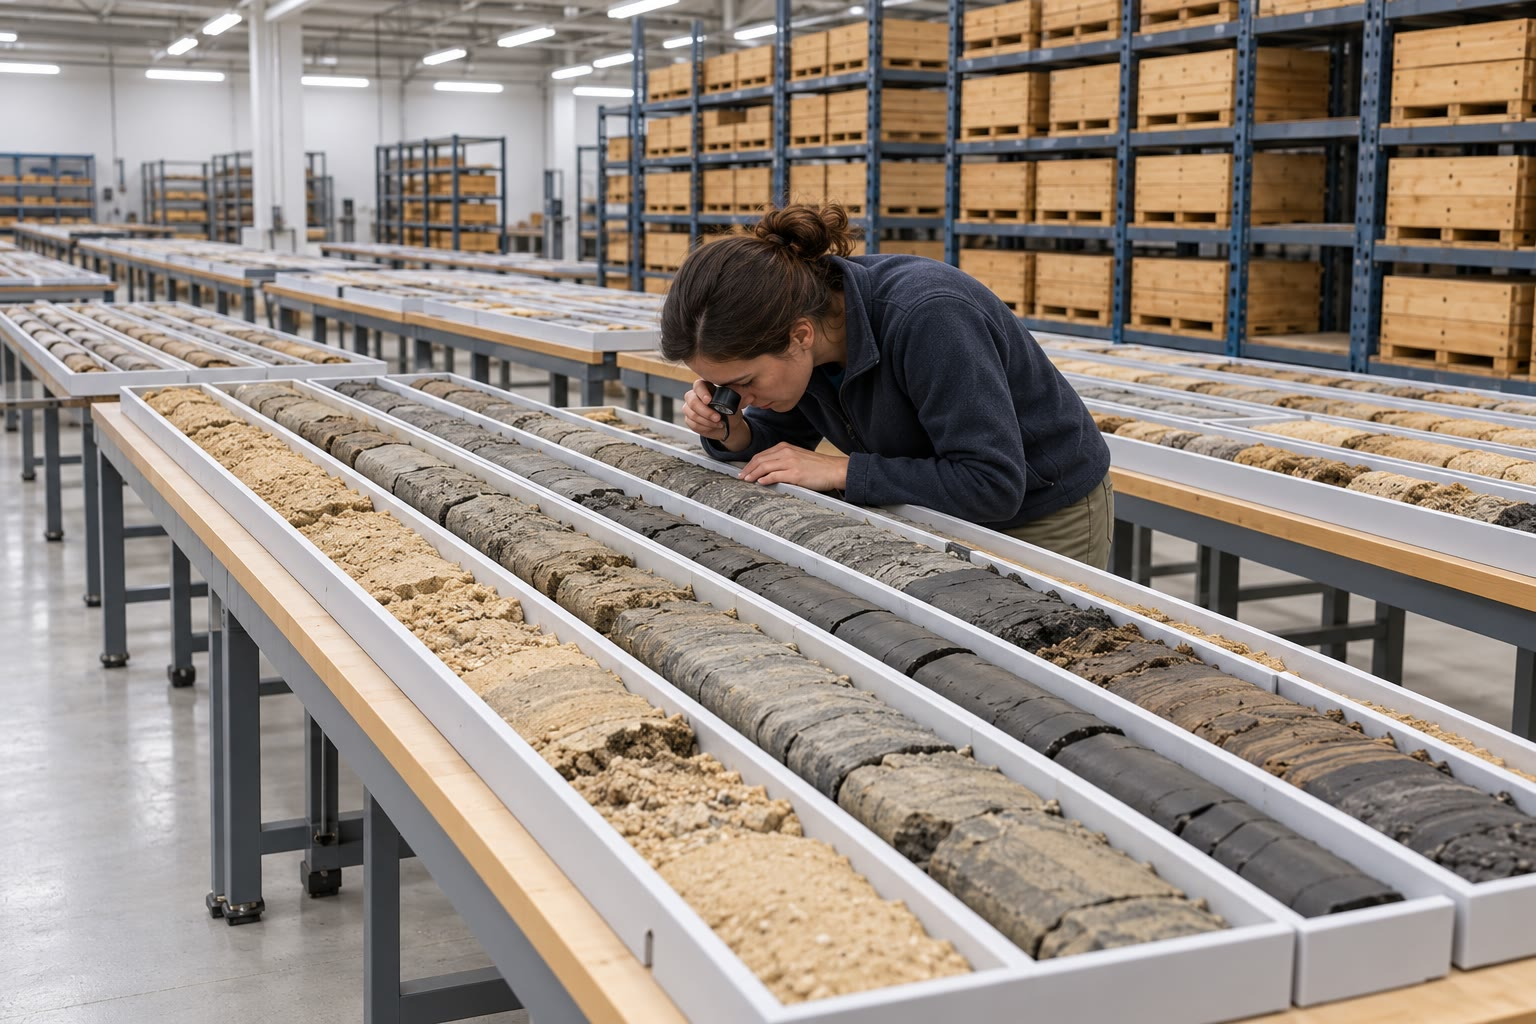
\includegraphics[width=\linewidth]{images/book5/ai/b3-core-store.jpg}

{\scriptsize Um depósito de testemunhos: testemunhos partidos de areia e lama em bandejas, um geólogo
com uma lupa de mão. Ilustração gerada por IA.}
\end{minipage}
\end{inthelab}

\section{Exercícios}

\begin{exercise}[$\star$]\label{exo:b3:facies-models:1}
Um testemunho mostra, da base para cima: lama de plataforma externa, lama intercalada com areia fina,
areia de \omterm{def:b3:facies-models:shoreface}{antepraia}, areia de praia, depois carvão com raízes. Usando a lei de Walther, dê a
ordem dos ambientes ao longo da costa na época e a direção
em que a linha de costa se deslocou. O que uma transgressão teria deixado?
\end{exercise}

\begin{exercise}[$\star$]\label{exo:b3:facies-models:2}
Três corpos arenosos apresentam formas de raios gama: (a) um sino com \qty{8}{m} de espessura e base
abrupta; (b) um funil com \qty{20}{m} de espessura; (c) um cilindro com \qty{30}{m}
de espessura, com topo e base abruptos. Sugira um ambiente para cada um, e a
observação em um testemunho que o confirmaria.
\end{exercise}

\begin{exercise}[$\star$]\label{exo:b3:facies-models:3}
Um arenito apresenta $\rho_b = \qty{2.40}{g/cm^3}$. Calcule a porosidade com uma
matriz de quartzo e água doce e, em seguida, com salmoura de \qty{1.1}{g/cm^3}.
\end{exercise}
% ledger: keys:density-porosity

\begin{exercise}[$\star$]\label{exo:b3:facies-models:4}
Ondas de comprimento de onda modal \qty{75}{m} e \qty{110}{m} (o mar abrigado e
o aberto do estudo com boias). Estime a profundidade em que cada uma mantém
\qty{4}{\percent} de seu movimento na superfície, e a fração que resta a uma profundidade de
\qty{20}{m}.
\end{exercise}
% ledger: losspeters10:wavebase

\begin{exercise}[$\star\star$]\label{exo:b3:facies-models:5}
Um calcário apresenta $\Delta t = \qty{60}{\micro\second/ft}$. Calcule sua
porosidade com a equação do tempo médio para uma matriz de 47.6 e de
\qty{52.6}{\micro\second/ft} e salmoura com \qty{189}{\micro\second/ft}. O que
a diferença ensina?
\end{exercise}
% ledger: keys:sonic

\begin{exercise}[$\star\star$]\label{exo:b3:facies-models:6}
Um intervalo de \qty{40}{m} contém camadas de areia de 6.0, 3.5, 8.0 e \qty{2.5}{m}
abaixo do valor de corte, sendo o restante lama. Calcule sua \omterm{def:b3:facies-models:ntg}{razão net-to-gross}. Com uma
porosidade de \qty{22}{\percent} na areia, quanto volume de poros contém um
quilômetro quadrado do intervalo?
\end{exercise}

\begin{exercise}[$\star\star$]\label{exo:b3:facies-models:7}
Uma camada de turbidito próxima à boca de um cânion tem \qty{1.2}{m} de areia maciça
(Ta) erodida no topo pela camada seguinte; \qty{30}{km} abaixo do leque, uma camada do
mesmo fluxo tem \qty{8}{cm} de areia fina e silte com laminação ondulada sob
\qty{3}{cm} de lama. Nomeie as divisões de cada uma e explique a mudança.
\end{exercise}

\begin{exercise}[$\star\star$]\label{exo:b3:facies-models:8}
Uma \omterm{def:b3:facies-models:association}{sucessão com granodecrescência ascendente} de \qty{9}{m} de espessura tem uma base abrupta com seixos,
areia com estratificação cruzada, areia fina ondulada e lama com raízes. Interprete-a e
estime a profundidade do canal que a construiu. A lei de Walther pode ser aplicada através de
sua base? Por quê?
\end{exercise}

\begin{exercise}[$\star\star$]\label{exo:b3:facies-models:9}
Um assoalho de plataforma desce \qty{60}{m} ao longo de \qty{40}{km}; outro mantém uma
profundidade de \qty{5}{m} por \qty{30}{km}, depois desce \qty{300}{m} ao longo de
\qty{1.5}{km}. Calcule os dois gradientes, nomeie cada plataforma e as fácies
esperadas na borda da segunda.
\end{exercise}

\begin{exercise}[$\star\star\star$]\label{exo:b3:facies-models:10}
Uma linha de costa progradaria com velocidade $v$ enquanto o nível relativo do mar sobe a uma taxa
$A$, e seu cinturão de \omterm{def:b3:facies-models:shoreface}{antepraia} tem largura $w$. Mostre que a areia de \omterm{def:b3:facies-models:shoreface}{antepraia} na
sucessão vertical tem espessura $h = wA/v$. Calcule-a para $w = \qty{2}{km}$,
$A = \qty{0.2}{m/kyr}$ e $v = \qty{20}{m/kyr}$, e diga o que acontece quando
$A = 0$. Compare com a proposição sobre a \omterm{def:b3:sequence-stratigraphy:trajectory}{trajetória da linha de costa} do
Capítulo~\ref{ch:b3:sequence-stratigraphy}.
\end{exercise}

\begin{exercise}[$\star\star\star$]\label{exo:b3:facies-models:11}
Um arenito apresenta $\rho_b = \qty{2.30}{g/cm^3}$ e $\Delta t =
\qty{86}{\micro\second/ft}$. Calcule sua porosidade a partir de cada perfil com uma matriz
de arenito de quartzo (2.65, \qty{52.6}{\micro\second/ft}) e salmoura (1.0 para a
densidade, \qty{189}{\micro\second/ft}). Se a porosidade sônica estiver correta, que
densidade de grão o \omterm{def:b3:facies-models:wireline}{perfil de densidade} implica, e o que pode ser o cimento?
\end{exercise}
% ledger: keys:density-porosity, keys:sonic

\begin{exercise}[$\star\star\star$]\label{exo:b3:facies-models:12}
Em um testemunho, lama marinha preta repousa diretamente sobre um carvão com raízes, com uma
fina camada de detritos de conchas no contato. Explique por que a lei de Walther não se
aplica através dele, qual superfície é essa e quanto da sucessão costeira
pode estar ausente se as ondas erodiram o assoalho até uma \omterm{def:b3:facies-models:shoreface}{base das ondas de tempo bom}
de cerca de \qty{10}{m} à medida que a linha de costa passava.
\end{exercise}

\section{Problema: Varden-2, um poço através da cobertura}

\begin{problem}[{Problema de fim de semana --- os perfis, a porosidade, as fácies e a areia líquida
de um poço inventado no sinclinal de Varden}]
\label{pb:b3:facies-models:1}
O poço Varden-2 é perfurado no sinclinal das Colinas de Varden, em
(7500, 7000) na malha da região, a partir de uma elevação do terreno de
\qty{441.0}{m}, até uma profundidade total de \qty{1200}{m}. Seus perfis estão desenhados na
figura da última seção. Use densidades de grão de 2.65 (quartzo) e
\qty{2.71}{g/cm^3} (calcita), uma água de poro de \qty{1.0}{g/cm^3}, tempos de trânsito da matriz
de 52.6 (arenito) e \qty{47.6}{\micro\second/ft}
(calcário), e \qty{189}{\micro\second/ft} para a água.

\medskip\noindent\textbf{Parte I --- Leitura dos perfis.}
\begin{enumerate}
\item O \omterm{def:b3:facies-models:wireline}{perfil de raios gama} salta de 12 para \qty{110}{API} em \qty{766}{m}, cai
  para 18 em \qty{866}{m}, torna-se irregular a partir de \qty{1046}{m} e estável em
  \qty{85}{API} a partir de \qty{1166}{m}. Nomeie as unidades atravessadas, usando seus perfis.
\item Calcule a espessura de cada unidade da cobertura e a elevação da
  base da cobertura.
\item O giz apresenta \qty{2.03}{g/cm^3} perto da superfície e
  \qty{2.36}{g/cm^3} a \qty{750}{m}. Calcule sua porosidade nas duas profundidades.
  O que acontece ao giz com a profundidade?
\item Por que não se atribui porosidade ao folhelho a partir de sua densidade?
\item O xisto apresenta \qty{2.75}{g/cm^3} e \qty{50}{\micro\second/ft}.
  O que o embasamento rápido, denso e não poroso diz ao perfurador?
\end{enumerate}

\medskip\noindent\textbf{Parte II --- Porosidade.}
\begin{enumerate}[resume]
\item O calcário apresenta \qty{2.573}{g/cm^3}: calcule sua porosidade por densidade.
\item Ele apresenta \qty{58.9}{\micro\second/ft}: calcule sua porosidade sônica e
  compare-a com a obtida pela densidade.
\item A areia limpa dos preenchimentos de canal apresenta \qty{2.32}{g/cm^3}: calcule
  sua porosidade.
\item Verifique-a com seu tempo de trânsito, \qty{79.9}{\micro\second/ft}.
\item Se a água de poro fosse uma salmoura de \qty{1.1}{g/cm^3}, em quanto mudaria
  a porosidade por densidade da areia?
\item Qual unidade faria o melhor aquífero ou reservatório, e qual seria o
  selante acima dela?
\end{enumerate}

\medskip\noindent\textbf{Parte III --- Fácies.} Um testemunho extraído de 1108 a
\qty{1124}{m} apresenta, da base para o topo: uma superfície erosiva com clastos de lama e
seixos; \qty{10.4}{m} de areia média com estratificação cruzada; \qty{3.2}{m} de areia fina com marcas onduladas
que passa a silte; \qty{2.4}{m} de lama marrom-avermelhada com vestígios de raízes.
\begin{enumerate}[resume]
\item Desenhe a forma esperada do \omterm{def:b3:facies-models:wireline}{perfil de raios gama} ao longo do intervalo recuperado em testemunho.
\item Identifique a sucessão e o ambiente de deposição de cada parte.
\item Com a lei de Walther, descreva os ambientes que se dispunham lado a lado.
\item Estime a profundidade do canal.
\item O arenito contém onze unidades desse tipo, cada uma sobre uma base abrupta. O que
  o empilhamento revela sobre o rio e sua planície?
\item A lei de Walther pode ser usada para passar de uma unidade para a seguinte? Por quê?
\end{enumerate}

\medskip\noindent\textbf{Parte IV --- Areia líquida.} Os onze preenchimentos de canal,
a partir da base do arenito, têm espessuras de 14, 9, 12, 7, 16, 10, 13, 8, 11, 12 e
\qty{8}{m}. Cada um começa com areia limpa (\qty{30}{API}) sobre uma fração
de sua espessura de 0.60, 0.45, 0.55, 0.30, 0.65, 0.40, 0.55, 0.35, 0.50,
0.45 e 0.30, depois granodecresce ao longo de uma fração de 0.25, 0.30, 0.25, 0.40,
0.20, 0.30, 0.25, 0.35, 0.25, 0.30 e 0.35, com a leitura de raios gama crescendo linearmente até
\qty{105}{API}, e termina em lama.
\begin{enumerate}[resume]
\item Qual fração de cada intervalo de granodecrescência fica abaixo do
  corte de \qty{60}{API}?
\item Calcule a areia líquida da unidade mais baixa e da mais espessa.
\item Calcule o total de areia limpa e o total dos intervalos de
  granodecrescência do arenito.
\item Calcule a \omterm{def:b3:facies-models:ntg}{razão net-to-gross}.
\item Como mudaria a areia líquida com um corte de 45 ou de
  \qty{75}{API}?
\item Com a porosidade da areia da questão 8, calcule o volume poroso da
  areia líquida sob um quilômetro quadrado.
\item Informe a espessura de areia líquida do arenito triássico em Varden-2.
\end{enumerate}
\end{problem}
% ledger: keys:density-porosity, keys:sonic, keys:gamma
